Graphiquement, nous représentons l'évolution de la probabilité de travailler pour une femme aux États-Unis (en 1975) lorsque nous faisons évoluer le nombre d'année d'expérience dans le poste actuel. 

\begin{figure}[!h]
    \caption{Évolution de la probabilité, de la côte et du odd-ratio de travailler pour une femme en fonction du nombre d'années d'expérience dans le poste actuel.}
    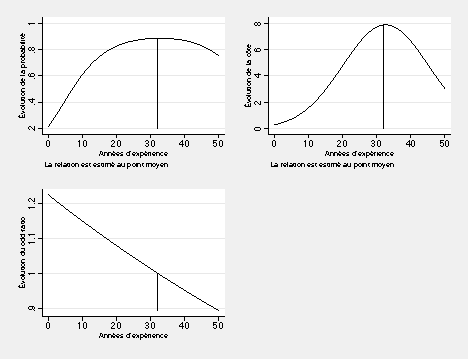
\includegraphics[scale = 1.5]{101_graphics/EvoProbaExperience.pdf}
    \centering
    \label{fig:EvolutionDelaProbabilitéEnFonctionDesAnnées}
\end{figure}

De manière évidente dans la figure \ref{fig:EvolutionDelaProbabilitéEnFonctionDesAnnées}, la relation n'est pas linéaire, elle a la forme d'une cloche (une fonction concave). Cela signifie que jusqu'à un certain seuil, une année d'expérience supplémentaire dans le poste actuel accroit la probabilité de participer au marché du travail, après, une année supplémentaire fait diminuer la probabilité supplémentaire de travailler. 

\vspace*{0.3cm}

Pour le calcul du seuil, c'est-à-dire le niveau où une année d'expérience supplémentaire n'accroit plus la probabilité de travailler, nous cherchons le niveau d'expérience qui donne un \emph{odd-ratio} égal à 1, alors nous posons les opérations suivantes : 
 
\begin{align}
    OR_{experience} & =  \frac{\frac{p_1}{1-p_1}}{\frac{p_0}{1-p_0}}  =  \frac{p_1}{1-p_1} \cdot \frac{1-p_0}{p_0}  = 1 & \nonumber \\
    % ou OR_{experience} & =  \frac{p_1}{1-p_1} \cdot \frac{1-p_0}{p_0}     = 1 & \nonumber\\
    & =  e^{\beta_1 + 2 \cdot \beta_2 \cdot exper_{seuil} + \beta_2} =1 & \nonumber \\
    log(OR_{experience}) & =  \beta_1 + 2 \cdot \beta_2 \cdot exper_{seuil} + \beta_2 = 0  &\nonumber \\ 
    exper_{seuil} & =  - \frac{\beta_1 + \beta_2}{2 \cdot \beta_2} \nonumber
\end{align}

En remplaçant les coefficients par leur valeur trouvée dans la régression Logit, nous pouvons en déduire les résultats suivants : 


\begin{align}
    &exper_{seuil} =  32.13 \nonumber \\
    &p_{seuil} = 12.34 \nonumber 
\end{align}
